%Language: LaTeX
%Author: Cong Liu (cong.liu20@imperial.ac.uk)
%Script: Report.tex
%Work directory: CMEECourseWork/Week3/Code
%Description: Report of the miniproject in thermal performance curves.

%Word Count


\documentclass[11pt]{article}

\usepackage{setspace}
\usepackage[colorlinks]{hyperref}
\usepackage{lineno}
\usepackage{booktabs}
\usepackage{graphicx}
\usepackage{float}
\usepackage{subfigure}
\usepackage[justification=centering]{caption}

\title{Model Selection to Find a Most Sufficient Model Fitting to Thermal Performance of Metabolic Traits\footnotemark[1]}

\author{Cong Liu\footnotemark[2]}

\renewcommand{\thefootnote}{\fnsymbol{footnote}}
\footnotetext[1]{Word Count: 2611}
\footnotetext[2]{Department of Life Sciences (Silwood Park), Imperial College of Science, Technology and Medicine}

\date{Nov, 2020}

\linespread{1.5}
\begin{document}
  \maketitle
  \newpage
    
  \linenumbers
  \begin{abstract}
    Determining thermal dependence of biological traits provides better understanding in distribution patterns of species 
    and is helpful in assessing the impact of climate change on biological systems. Here, I fitted quadratic polynomial 
    model, cubic polynomial model, Briere model and Ratkowsky model to observed data of metabolic traits under different 
    temperatures to calculate thermal performance curves. Model averaging and selection by either AIC or BIC were 
    conducted to find one most sufficient model fitting to empirical data of each curve. 
    In most curves, AIC and BIC give support to 
    the same model and Ratkowsky model has the highest frequency of being the most suitable model 
    under two selection criteria. However, for some thermal performance curves in the dataset, even the best model 
    selected here fail in describing thermal dependence of metabolic traits, indicating that the four plausible models 
    are not suitable and more models need to be involved. Overall, the results show that Ratkowsky model is sufficient 
    for most thermal performance curves involved in this study.

  \end{abstract}

  \section{Introduction}

  Temperature is an important abiotic factor that influences the functioning of organisms, especially 
  for ectotherms whose body temperatures reflect that of their environments to different extent. It affects 
  the rates of biochemical reactions and consequently has profound influence on different biological 
  activities like metabolism, growth, development and reproduction \cite{sinclair2016can}. And this can 
  lead to further consequences in abundance and distribution of organisms \cite{schulte2011thermal}. 
  Besides, interactions among species are also affected by thermal environment \cite{grigaltchik2012thermal}.  
  \newline
  Thermal performance curve describes the dependence of performance (usually, the rate of a physiological 
  activities or fitness) on temperature quantitatively \cite{sinclair2016can}. Generally, organisms response 
  to temperature fluctuation in a similar manner. The value of performance peaks at some temperature point, 
  and decreases when temperature deviates from the maximum point, while extremely high or low temperatures are lethal 
  \cite{sinclair2016can,krenek2011thermal}. 
  The mathematical modelling of thermal performance curve provides a framework for the estimation of 
  physiological characters like the optimum temperature at which performance peaks, upper and lower 
  thermal limit thermal performance, and thermal tolerance range \cite{krenek2011thermal}. 
  Besides, it is also helpful in predicting 
  performance of organisms when temperature fluctuates. Thus, thermal performance curve is helpful in better 
  understanding distribution patterns of species. There is evidence that 
  the thermal tolerance range of a species is often corresponded 
  to the temperature fluctuation of its habitat, indicating the 
  importance of temperature as a selective force in shaping distribution pattern \cite{sunday2011global, clusella2011climatic}. 
  There is also evidence showing 
  that thermal sensitivity plays a role in the dynamics of biodiversity \cite{allen2002global}. Furthermore, 
  investigations in thermal performance curve help better predict the impact of current climate change on 
  biological process \cite{krenek2011thermal, sears2011introduction}.  
  \newline
  Currently, there are numerous mathematical models with different properties  
  that are used to illustrate thermal performance curves of different clades 
  \cite{krenek2011thermal,angilletta2006estimating}. Which model, or models are sufficient in describing thermal dependence 
  of performance is the main concern of this study. 
  Using a dataset of observed data from 841 thermal performance curves, 
  I calculated these curves by fitting 
  four plausible models to them. 
  Then I conducted model averaging and selection to find one model that is most sufficient to describe the observed data.
   Akaike information criterion (AIC) or 
  Bayesian information criterion (BIC) was used as model selection criterion \cite{johnson2004model}. 
  Besides, whether metabolic trait or habitat type is corresponded to models that get most support from 
  empirical data was assessed.

  \section{Materials and Methods}
    \subsection{Original Data}
    The original dataset used here is named as ThermRespData.csv and its field names are defined in another 
    file called BiotraitsTemplateDescription.pdf. Both files are accessible in 
    \newline 
    \href{https://github.com/mhasoba/TheMulQuaBio/tree/master/content/data}{https://github.com/mhasoba/TheMulQuaBio/tree/master/content/data}. 
    \newline 
    The main fields of interest are OriginalTraitValue (trait values) and ConTemp (the temperatures 
    in Celsius scale). Each thermal performance curve is corresponded to a unique ID from 1 to 903. 
    Among them 62 curves contain negative trait values and were removed. 
    So a total of 841 thermal performance curves was used in following analysis. 
    
  \subsection{Plausible Models} 
    Denote by \textit{B} the trait value and \textit{T} the temperature. The function that describes 
    the relationship between temperature and trait value is  
    \begin{equation} 
      B = B(T) 
    \end{equation} 
    Plausible models are: (1) quadratic polynomial model with constants  
    $B_0$, $B_1$ and $B_2$: 
    \begin{equation} 
    B(T) = B_0 + B_1 T + B_2 T^2 
    \end{equation} 
    (2) cubic polynomial model with constants  
    $B_0$, $B_1$, $B_2$ and $B_3$: 
    \begin{equation} 
    B(T) = B_0 + B_1 T + B_2 T^2 + B_3 T^3 
    \end{equation} 
    (3) Briere model with constants  
    $B_0$, $T_0$ and $T_m$ 
    \cite{briere1999novel}: 
    \begin{equation}\label{equ:Briere} 
    B(T) = B_0 T (T - T_0) \sqrt{T_m - T} 
    \end{equation} 
    $T_0$ and $T_m$ are lower and upper thermal limit thermal performance. 
    \newline 
    (4) Ratkowsky model with constants  
    $T_0$, $T_m$, $a$ and $b$  
    \cite{ratkowsky1983model}: 
    \begin{equation} 
    B(T) = \{a (T-T_0) (1-e^{b(T-T_m)})\}^2 
    \end{equation} 
    $T_0$ and $T_m$ are lower and higher thermal limit thermal performance. 
  \subsection{Model Fitting} 
    To conduct model fitting, least square method was used, and non-linear models were fitted using Levenberg-Marquardt  
    algorithm \cite{ranganathan2004levenberg, lourakis2005brief}. Maximum iteration number was 200.  
    \newline 
    For fitting of Briere model, start values of $T_0$ and $T_m$ were the lowest and highest sampled temperatures 
    of each curve and they are denoted by $T_{0st}$ and $T_{mst}$ respectively. From Eq. (\ref{equ:Briere}), 
    \begin{equation}\label{lalala} 
    B_0 = \frac{B(T)}{T (T - T_0) \sqrt{T_m - T}} 
    \end{equation} 
    For each curve, remove samples with lowest and highest temperatures and denote the rest as  
    $\{(T_i, B_i), i = 1,2,\cdots,n-2\}$, where $n$ is sample size.  
    So from Eq. (\ref{lalala}), a rough estimation of $B_0$, denoted by $B_{0est}$ can be given by  
    \begin{equation}\label{esti} 
    B_{0est} = \frac{\sum_{i=1}^{n-2}\frac{B_i}{T_i (T_i - T_{0st}) \sqrt{T_{mst} - T_i}}}{n-2} 
    \end{equation} 
    The start values of $B_0$ was taken from a uniform distribution between $0$ and $2B_{0est}$. 
    Each curve was fitted 100 times with different start values of $B_0$. 
    \newline 
    As for fitting of Ratkowsky model, start values of $T_0$ and $T_m$ were the lowest and highest sampled temperatures 
    of each curve. Start values of $a$ and $b$ were taken from set  
    $\{10^i: i = -5,-4,-3,-2,-1,0,1,2,3,4\}$. So for each curve, there are ten start values of $a$ and $b$,  
    and 100 combinations of them. Hence, each curve was fitted 100 times with different start values.

  \subsection{Model Selection}
  After model fitting, AIC and BIC of all models  
  were calculated using  
  following equations \cite{johnson2004model}: 
  \begin{equation} 
  AIC = -2L + 2k 
  \end{equation} 
  \begin{equation} 
  BIC = -2L + klnn 
  \end{equation} 
  where $n$ is sample size, $k$ is number of parameters in the model, and $L$ is maximized log-likelihood value of the model. 
  $L$ is given by the following equation \cite{johnson2004model}: 
  \begin{equation} 
  L = -\frac{n}{2}ln\frac{RSS}{n} 
  \end{equation} 
  where $RSS$ is residual sum of squares of the model. 
 
  \subsection{Model Averaging}
  In non-linear model fitting, dataset for each thermal performance curve was fitted 100 times and multiple solutions 
  with similar AIC or BIC could 
  be obtained. To find one most sufficient model supported by observed data, I conducted model averaging. 
  Among all solutions obtained through dataset of one thermal performance curve, those with lowest AIC or BIC values 
  were selected and averaged. 
  For one thermal performance curve, denote by $l$ the number of optimal solutions with lowest AIC or BIC among all solutions 
  obtained 
  by non-linear model fitting, and $\theta_i$ the $i$th solution, then the parameters of averaged model, denoted by $\theta$, 
  is given by following equation \cite{johnson2004model, buckland1997model}:
  \begin{equation}
    \theta = \sum_{i=1}^{l}\omega_i\theta_i
  \end{equation}
  The weight $\omega_i$ is given by smoothed AIC or BIC method \cite{buckland1997model}:
  \begin{equation}
    \omega_i = \frac{e^{-xIC_i/2}}{\sum_{i=1}^{l}e^{-xIC_i/2}}
  \end{equation}   
  where $xIC_i$ is the AIC or BIC of $i$th solution. Here, model averaging was conducted to solutions with equal AIC 
  or BIC values, 
  so 
  \begin{equation}
    \omega_i = \frac{1}{l}
  \end{equation}
  Then I calculated AIC and BIC of the averaged model and conducted model selection among linear and non-linear models.
  
  
  \subsection{Computating Tools}
  Most scripts are written in R 4.0.3, taking advantage of its powerful packages in model fitting 
  and visualization, and of in-built functions for form processing. R package minpack.lm was used for model 
  fitting, while visualization was conducted by R packages ggplot2, gridExtra and cowplot. 
  The report was written using LaTeX because it is efficient in typesetting. 
  A bash script was used to compile LaTeX source code. 
  Finally, a python3 script was written to run all scripts using os module. 

  \section{Results}
    \subsection{Model Fitting and Selection}
    For each curve, models with lowest AIC or BIC were selected and they are either quadratic, 
    cubic, of Briere or of Ratkowsky. No curve has multiple models equally supported by AIC or BIC. 
    Among 841 thermal performance curves, 639 (76.0\%) of them can be fitted by Briere model, and 649 (77.2\%) of them can 
    be fitted by Ratkowsky model. After model fitting, Briere or Ratkowsky models with lowest AIC or BIC 
    values among all solutions 
    were selected and averaged before further model selection. 
    Figure. 1 provides examples of models that were used in selection among linear and non-linear models, and Figure 2 
    illustrates the distributions of AIC and BIC for each curve.
    \begin{figure}[H]
      \centering
      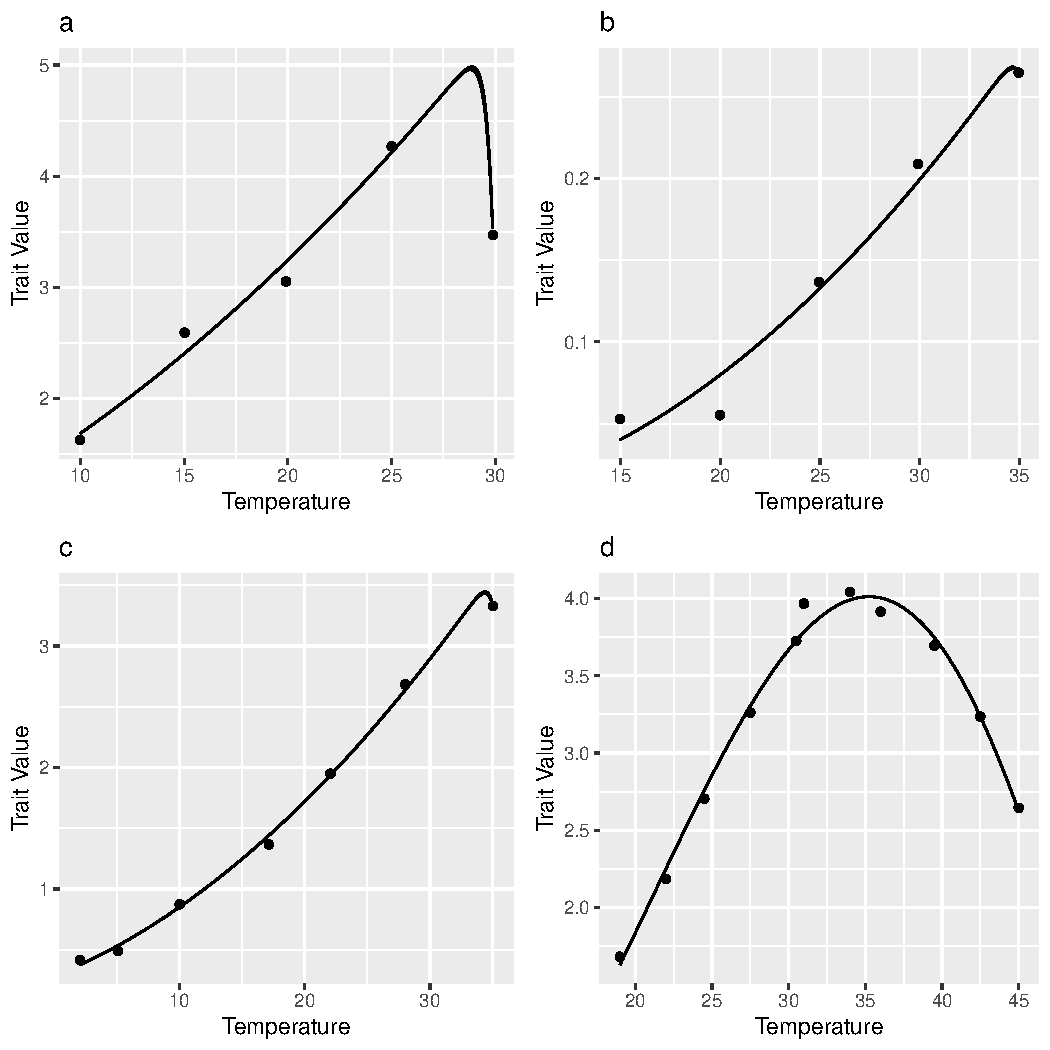
\includegraphics[width=\textwidth]{../Results/Fig1.pdf}
      \caption{Examples of models used for model selection. Criterion of selection within non-linear models is AIC for 
      subfigure \textbf{a}, \textbf{b} and \textbf{c}; and BIC for subfigure \textbf{d}, \textbf{e} and \textbf{f}. 
      The IDs of thermal performance curves 
      are: 148 (\textbf{a}), 204 (\textbf{b}), 322 (\textbf{c}), 138 (\textbf{d}), 237 (\textbf{e}),
      519 (\textbf{f}).}
    \end{figure}

    \begin{figure}[H]
      \centering
      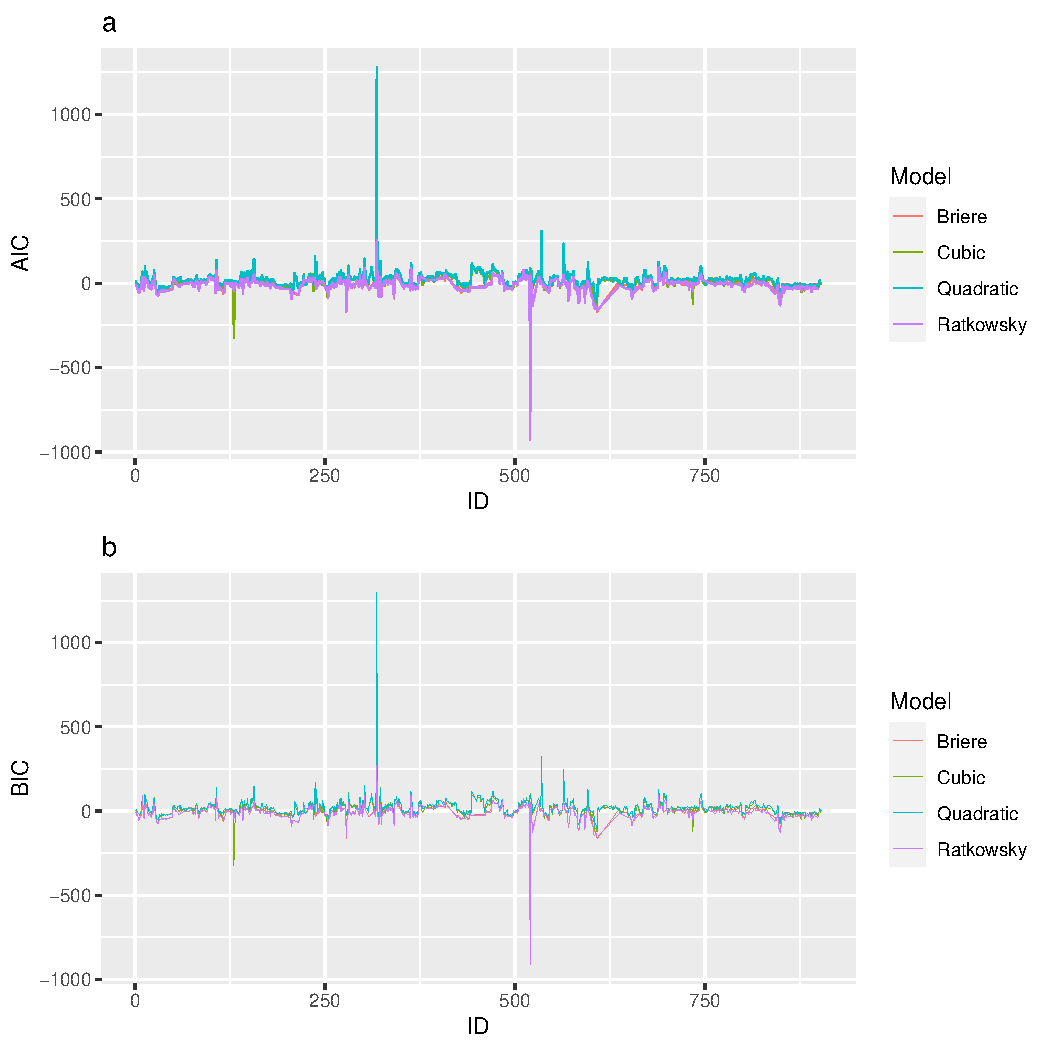
\includegraphics[width=\textwidth]{../Results/a.pdf}
      \caption{The distribution of AIC and BIC. The lateral axis represents the IDs of curves, and the vertical 
      axis represents values of AIC (\textbf{a}) or BIC (\textbf{b}). The colours of lines represent different 
      plausible models.}
    \end{figure}
    When AIC is used as criterion for model selection, 57 (6.78\%) curves are  
    fitted by quadratic polynomial function and 160 (19.02\%) curves for cubic polynomial function. As for non-linear 
    models, 190 (22.59\%) curves are fitted by Briere model, and the rest 434 (51.61\%) curves are fitted by Ratkowsky 
    model. When BIC is used for model selection, 218 (25.92\%) curves are fitted by linear models (55 quadratic 
    polynomial model and 163 cubic polynomial model). 191 (22.71\%) curves are fitted by Briere model, while the 
    rest 432 (51.37\%) curves are fitted by Ratkowsky model. 18 curves are sufficiently 
    fitted by different models under different criteria for model selection as shown in Table 1.
    \begin{table}[H]
      \centering
      \caption{Curves That AIC and BIC Support Different Models}
      \begin{tabular}{@{}cccc@{}}
        \toprule
        ID  & AIC-supported   & BIC-supported \\ \midrule
        99  & Briere    & Ratkowsky \\
        105 & Ratkowsky & cubic     \\
        232 & Ratkowsky & Briere              \\
        318 & Ratkowsky & Briere            \\
        330 & Briere    & Ratkowsky           \\
        351 & Briere    & Ratkowsky           \\
        426 & Ratkowsky & Briere             \\
        496 & Briere    & Ratkowsky          \\
        569 & Ratkowsky & Briere             \\
        635 & quadratic & cubic               \\
        644 & quadratic & cubic               \\
        669 & Ratkowsky & Briere             \\
        681 & Ratkowsky & Briere             \\
        737 & Briere    & Ratkowsky           \\
        745 & Ratkowsky & Briere             \\
        765 & Briere    & Ratkowsky           \\
        827 & Ratkowsky & Briere              \\
        879 & Briere    & Ratkowsky           \\ \bottomrule
        \end{tabular}
        \end{table}

        \subsection{Assess Best Models for Curves of Different Metabolic or Habitat Types}
        To assess preferred models for thermal performance curves of differnet metabolic traits or species living in different 
        habitat types, 18 curves were removed because AIC and BIC supported different models. So a total of 823 
        curves were involved.
        \newline  
        In the original dataset, the metabolic trait of each curve is defined in the field of StandardisedTraitName 
        (trait name for comparison), 
        which contains three categories: gross photosynthesis rate, net photosynthesis rate and respiration rate. Another field 
        relevant to 
        trait name is OriginalTraitName (trait name as it found in source). It should be noted there are four curves 
        have no StandardisedTraitName, while their OriginalTraitName are oxygen evolution 
        rate in thylakoid membranes (IDs: 698, 699) and cell specific photosynthesis rate (IDs: 441, 442). They were not 
        involved in assessing which model is suitable for different metabolic traits.
        As for habit type of each curve, it is defined in another field (Habitat), which is composed of four types: aquatic, 
        freshwater, freshwater/terrestrial, marine and terrestrial. Here I assessed which model is suitable for determining 
        thermal performance of species living in terrestrial or non-terrestrial (aquatic, 
        freshwater, freshwater/terrestrial and marine) habitats.
        \newline  
        Table 2 illustrates the sufficient models for thermal performance curves of different metabolic traits. 
        A total of 819 thermal performance curves of three metabolic traits are involved. 
        For models of each metabolic trait, non-linear  
        model occupies a larger proportion 
        (75.0\% of gross photosynthesis rate, 78.8\% of net photosynthesis rate, and 66.2\% of respiration rate) than linear 
        models. Besides, Ratkowsky model takes a bigger amount than Briere model in all metabolic traits except gross 
        photosynthesis rate.
        \newline
        Then I classified thermal performance curves according to whether the species studied is specific in terrestrial 
        habitats (Table 3). Non-linear model 
        takes the biggest amount of sufficient models for both two kinds of habitat type 
        (82.1\% for terrestrial habitat and 55.2\% of non-terrestrial habitat), and Ratkowsky model occupies biggest proportion 
        among four models. 
        \begin{table}[H]
          \centering
          \caption{Selected Models for Thermal Performance Curves of Different Metabolic Traits}
          \begin{tabular}{@{}ccccc@{}}
          \toprule
          Model     & Gross photosynthesis rate & Net photosynthesis rate & Respiration rate  & Total \\ \midrule
          Quadratic & 0   & 19  & 36  & 55    \\
          Cubic     & 9   & 80  & 71  & 160   \\
          Briere    & 16  & 73  & 94  & 183   \\
          Ratkowsky & 11  & 294 & 116 & 421   \\
          Total     & 36  & 466 & 317 & 819   \\ \bottomrule
          \end{tabular}
          \end{table}
      
      
          \begin{table}[H]
            \centering
            \caption{Selected Models for Thermal Performance Curves from Species in Different Habitat Types}
            \begin{tabular}{@{}cccc@{}}
            \toprule
            Model     & Terrestrial & Non-terrestrial & Total \\ \midrule
            Quadratic & 21          & 34              & 55    \\
            Cubic     & 81          & 79              & 160   \\
            Briere    & 134         & 49              & 183   \\
            Ratkowsky & 335         & 90              & 425   \\
            Total     & 571         & 252             & 823   \\ \bottomrule
            \end{tabular}
            \end{table}


    \subsection{Preferred Models May not Describe the Observed Data Well}
    Through model selection, I selected one model for each curve and it is the most sufficient one in terms of describing 
    the thermal performance curve among four plausible models. However, the preferred models of some curves still 
    fail in describing thermal performance throughout the temperature 
    range between lower and upper thermal limits of performance. As the growth of temperature in this range, 
    performance is supposed to increases, peaks at some point, and then drops \cite{sinclair2016can,krenek2011thermal}. 
    The preferred models of some curves are 
    not bell-shaped (Figure. 3). Furthermore, ecologically unrealistic estimations 
    of thermal limits of performance are also given by some selected models (Figure 4). 
     
    \begin{figure}[H]
      \centering
      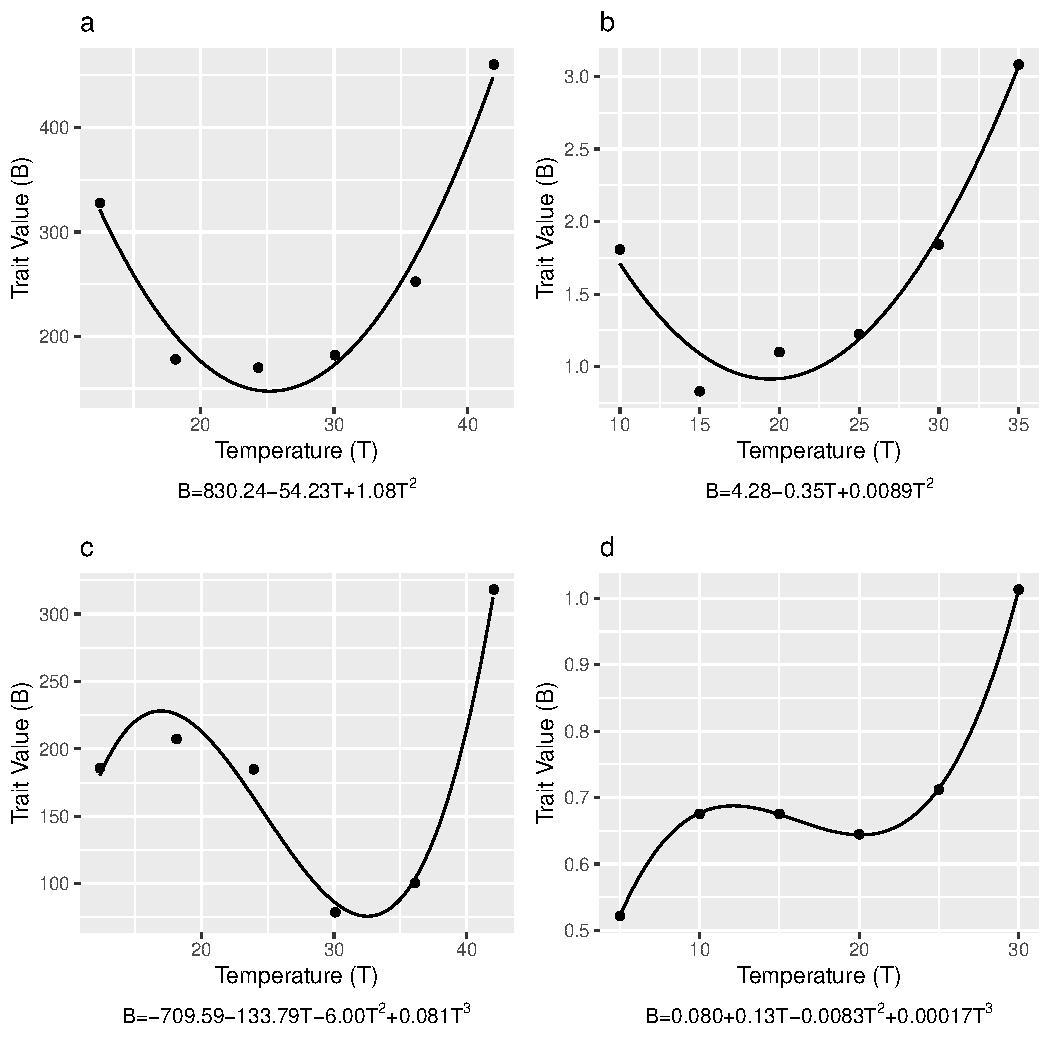
\includegraphics[width=\textwidth]{../Results/Fig2.pdf}
      \caption{Examples of preferred models that are not bell-shaped curves. IDs of thermal performance curves 
      are: 456 (\textbf{a}), 
      841 (\textbf{b}), 455 (\textbf{c}), 600 (\textbf{d}). Mathematical expression of each model is given at 
      the bottom of each subfigure. For these datasets, AIC and BIC support the same models with equal parameters.} 
    \end{figure}

    \begin{figure}[H]
      \centering
      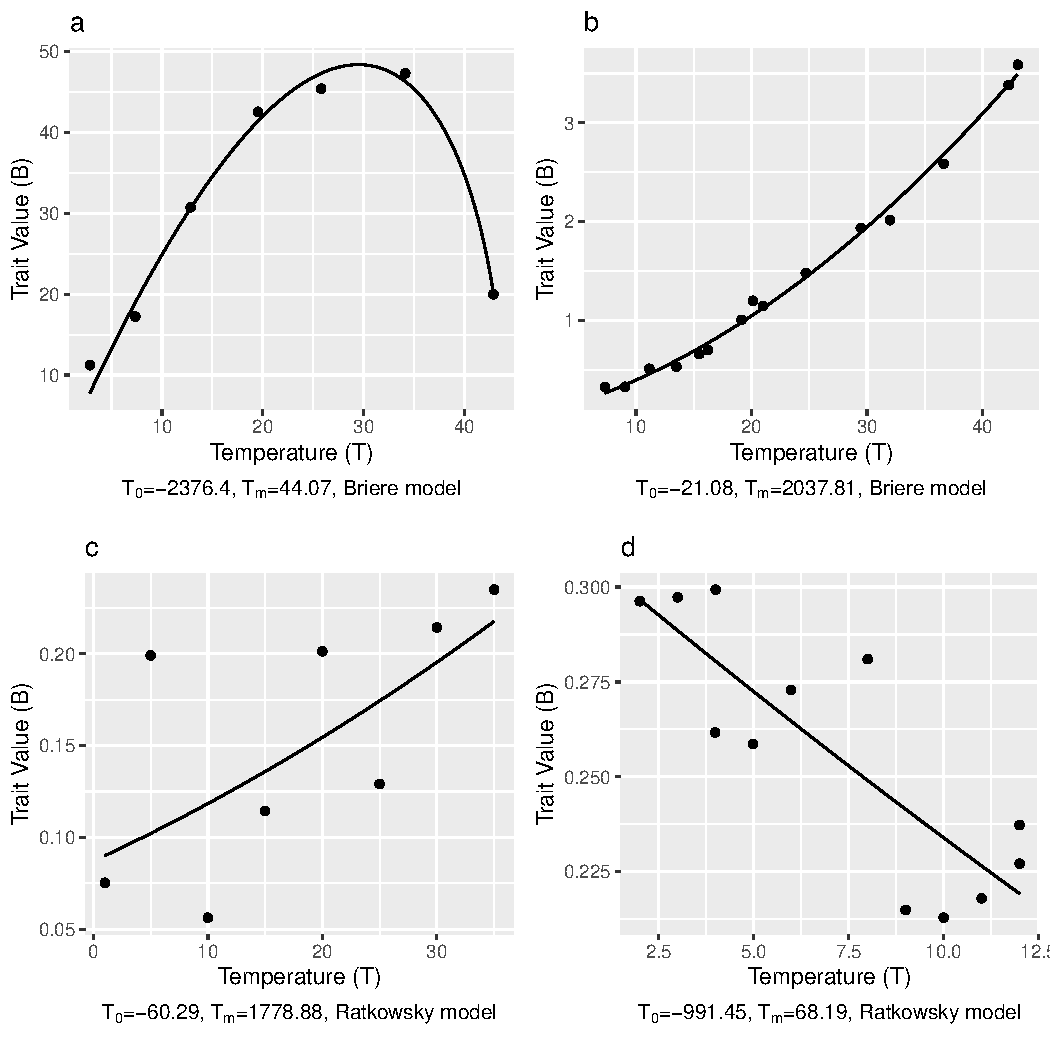
\includegraphics[width=\textwidth]{../Results/b.pdf}
      \caption{Examples of preferred models that give unrealistic estimations of thermal limits of performance. 
      IDs of thermal performance curves are: 81 (\textbf{a}), 
      215 (\textbf{b}), 46 (\textbf{c}), 254 (\textbf{d}). Criterion of model selection is AIC, and estimations of lower 
      and upper thermal limits of performance, denoted as $T_0$ and $T_m$, are given at the bottom of each subfigure.}
    \end{figure}

  
  \section{Discussion}
  Investigations in how organisms response to temperature fulctuation are helpful in better understanding 
  the impact of recent and future climate change on biological systems \cite{kingsolver2013heat, vasseur2014increased}. 
  In assessment of thermal performance, it is important to choose an appropriate mathematical model that 
  is best supported by empirical data and is able to provide relatively precise estimations of controlled variable, 
  given values of independent variable. Currently, there are plenty of mathematical models used in fitting thermal 
  performance curves, and model selection criteria can be used to explicate how sufficient a model is in describing 
  thermal performance curves \cite{krenek2011thermal, angilletta2006estimating, johnson2004model}. 
  In order to find which model is best supported by observed data of thermal performance, 
  I fitted four plausible models to a dataset composed of 841 thermal performance curves 
  and conducted model averaging and selection using either AIC or BIC as criterion. 
  In most cases, AIC and BIC prefer the same model.
  The results also showed that under both selection criteria, 
  Ratkowsky model is sufficient in quantifying thermal performance for about 51\% of curves in the dataset. 
  \newline
  In model selection, a set of plausible models are ranked by some criterion and the most appropriate one is selected. 
  AIC and BIC are two criterion for model selection. 
  They take 
  both fit and model complexity into consideration to balance under- and over-fitting to observed data 
  \cite{johnson2004model, zucchini2000introduction}. Although AIC and BIC are quite similar 
  in forms, they are divergent in theoretical motivations. BIC is based on Bayesian statistical analysis and is an 
  approximation reflecting the probability that each plausible model is the true model that generated the empirical 
  data \cite{kuha2004aic}. Minimized BIC is corresponded to maximized posterior 
  probability among all plausibilities and can be thought as a criterion for model selection \cite{wit2012all}. However, 
  the existence of "true model" is problematic \cite{box1979all}, and the theoretical basis of BIC is 
  controversial \cite{kuha2004aic}. As for AIC, it measures the predictive performance of 
  each candidate model by estimating Kullback-Leible information loss \cite{kuha2004aic,deleeuw1992akaike, 
   burnham2004multimodel}, 
  and is thus well-founded in information theory.  
  Here, I conducted model selection using AIC and BIC as criterion respectively. 
  In most cases, they prefer the same model. However, I tend to use AIC as model selection criterion because of its solid 
  theoretical foundation.
  \newline
  In non-linear model fitting, an iterative algorithm is employed to gain a numerical local optimal solution, 
  which is sensitive to start values 
  \cite{ranganathan2004levenberg, lourakis2005brief}. 
  Here, 
  I fitted each non-linear model 100 times with different start values before model selection, attempting to 
  find the global optimal solution. For one thermal 
  performance dataset, multiple solutions can be obtained by different start values while they have equal and 
  lowest AIC or BIC. This is because of limited accuracy in numerical calculation of AIC and BIC 
  by R scripts. To deal with this, I conducted model averaging using smoothed AIC or BIC method. 
  When multiple plausible models get nearly equivalent support from observed data (\textit{e.g.} similar AIC or BIC values), 
  model averaging is a good method 
  to give estimations of model parameters or predict values of response variables \cite{johnson2004model}.
  \newline
  Generally, thermal performance curve is supposed to be a bell-shaped curve with ecologically realistic 
  lower and upper thermal limits of performance \cite{sinclair2016can,krenek2011thermal}. 
  However, some models supported by AIC or BIC are not bell-shaped curves, 
  as exemplified in Figure 3. Others may give estimations of thermal limits of performance that are too low or too high to 
  be realistic, as exemplified in Figure 4. Such models may fit to the observed data well (Figure 3d and Figure 4a), but 
  fail in describing the whole thermal performance curve. A possible reason is that there are not enough sampes from a wide 
  enough temperature range to allow the models to capture the change of performance over temperature in different ranges. 
  For example, curve 215 
  only contains samples of relatively low temperature (\textit{i.e.} temperatures of all samples are no greater 
  than the optimum 
  temperature  
  where performance peaks) as it is shown in Figure 4b. An alternative explanation is that none of the four plausible models 
  are suitable for describing the observed data. 
  AIC and BIC can only explicate the relative goodness of each model in a given set of models \cite{johnson2004model, 
  buckland1997model, zucchini2000introduction}
   and it 
  is possible that no model in the given set can fit to the observed data sufficiently. Under these circumstances, more 
  models are needed to be used in fitting and selection.

  Overall, I conducted model fitting, averaging and selection using observed data of 841 thermal performance curves. 
  Plausible models include quadratic polynomial model, cubic polynomial model, Briere model and Ratkowsky model. AIC and 
  BIC were used as model selection criterion. For most curves, AIC and BIC give support to the same model. The results shows 
  that for more than a half of thermal performance curves involved here, Ratkowsky model is the most sufficient one among 
  four plausibilities. When curves are classified according to metabolic trait or habitat type of species, Ratkowsky model is 
  most sufficient one for a majority of curves in most categories. However, some selected models cannot describe the whole 
  thermal performance curves or contain unrealistic parameters, indicating that none of the four models is suitable for 
  fitting to the observed data.
  
  \newpage
  
  \bibliographystyle{unsrt}
  \bibliography{References}

\end{document}
